\chapter{Progettazione e codifica}
\label{cap:progettazione-codifica}

\section{Struttura dell'estensione}
\label{sec:struttura-estensione}

Come rappresentato in figura \ref{fig:struttura_estensione}, l’estensione si basa su tre componenti fondamentali: \textit{manifest.json}, \textit{service worker} \textit{(background script)} e \textit{content script}.

\subsection{Manifest.json}

Il file \textit{manifest.json} è il cuore dell’estensione: descrive il contenuto in un formato strutturato e definisce le regole per l'iniezione dei \textit{content script}.

\subsection{Service Worker}

Il \textit{service worker} è uno script \textit{singleton} che il browser esegue in background. Non ha accesso diretto alle pagine web, ma può interagire con esse tramite i \textit{content script}. Viene utilizzato per gestire gli eventi del browser (come la chiusura di una scheda o il clic sull’icona dell’estensione nella barra degli strumenti) e coordinare i componenti dell'estensione.

\subsection{Content Script}

I \textit{content script} sono file che vengono iniettati nelle pagine web ed eseguiti nel contesto di quelle stesse pagine. Possono visualizzare e manipolare il \gls{dom} in modo analogo agli script caricati da ciascuna pagina. Hanno accesso a un insieme limitato delle \gls{api} di WebExtension, che può essere esteso tramite la comunicazione con i \textit{background script}.

\begin{figure}[H]
  \centering 
  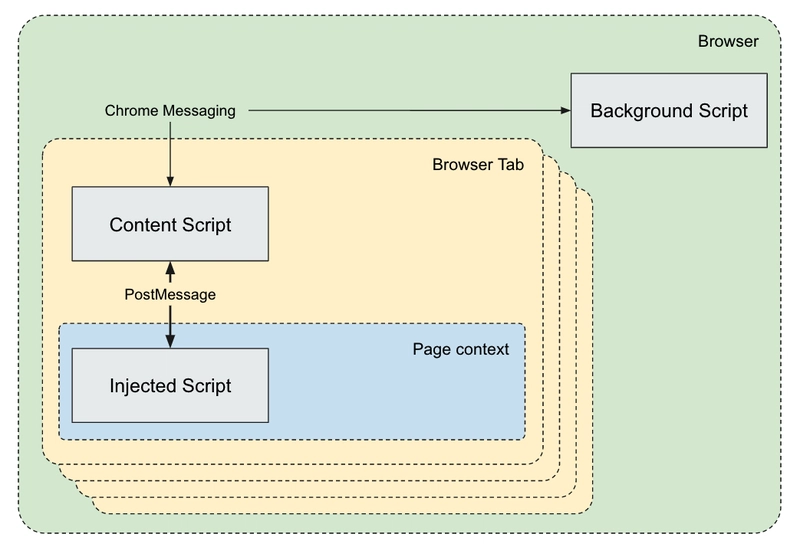
\includegraphics[width=0.8\columnwidth]{progettazione/estensione.png}
  \caption{Struttura dell'estensione}
  \label{fig:struttura_estensione}
\end{figure}

\section{Mockup dell'interfaccia grafica}
\label{sec:mockup}

Durante la progettazione dell’interfaccia grafica, ho tratto ispirazione da diverse soluzioni esistenti analizzate nella fase preliminare. In particolare:
\begin{itemize}
    \item Lo stile delle informazioni in anteprima (come meta keywords, conteggio delle parole e altri dati \gls{seo}) si ispira al layout dell’estensione \textit{Detailed SEO Extension}, al quale è stato aggiunto un comportamento flessibile per gestire dinamicamente lo spazio nella barra laterale;
    \item Il \textit{box} di inserimento della parola chiave è il risultato di una combinazione tra le interfacce di \textit{MozBar} e \textit{Wincher}. Da \textit{MozBar} ho ripreso l’idea della \textit{checkbox} posizionata sotto il campo di \textit{input}, che permette di evidenziare una parola chiave senza dover eseguire preventivamente una ricerca o un’analisi. \textit{Wincher}, invece, ha ispirato il design del campo di testo affiancato da un pulsante per avviare l’analisi;
    \item L’organizzazione delle parole chiave in categorie (user-added keywords, meta keywords, most frequent keywords) si basa su un approccio integrato derivato da strumenti come \textit{Keyword Density Analyzer}, \textit{SEOquake}, \textit{SEOptimer} e \textit{SEO tester online}. Da questi strumenti ho ripreso anche l’idea di una rappresentazione dei risultati in formato tabellare;
    \item Il sistema di filtraggio delle parole chiave - non presente nella prima bozza dell’interfaccia - è stato ispirato da \textit{SEOquake}, che offre funzionalità simili per agevolare la consultazione dei risultati.
\end{itemize}

\vspace{5pt}
\noindent Le scelte progettuali sopra elencate sono state accompagnate da un’analisi dello spazio disponibile e delle \textit{best practice} in materia di design, con l’obiettivo di definire fin dalle prime fasi quali elementi utilizzare e come disporli sull’interfaccia per garantire comfort visivo ed evitare il sovraccarico cognitivo. Per la scelta cromatica, il punto di partenza è stato il colore più distintivo, il viola, attorno al quale è stata costruita una combinazione di colori coerente e conforme alle linee guida \gls{wcag}. Questi concetti sono stati infine tradotti in un \textit{mockup}, realizzato con Figma e riportato in figura \ref{fig:mockup}.

\begin{figure}[H]
  \centering 
  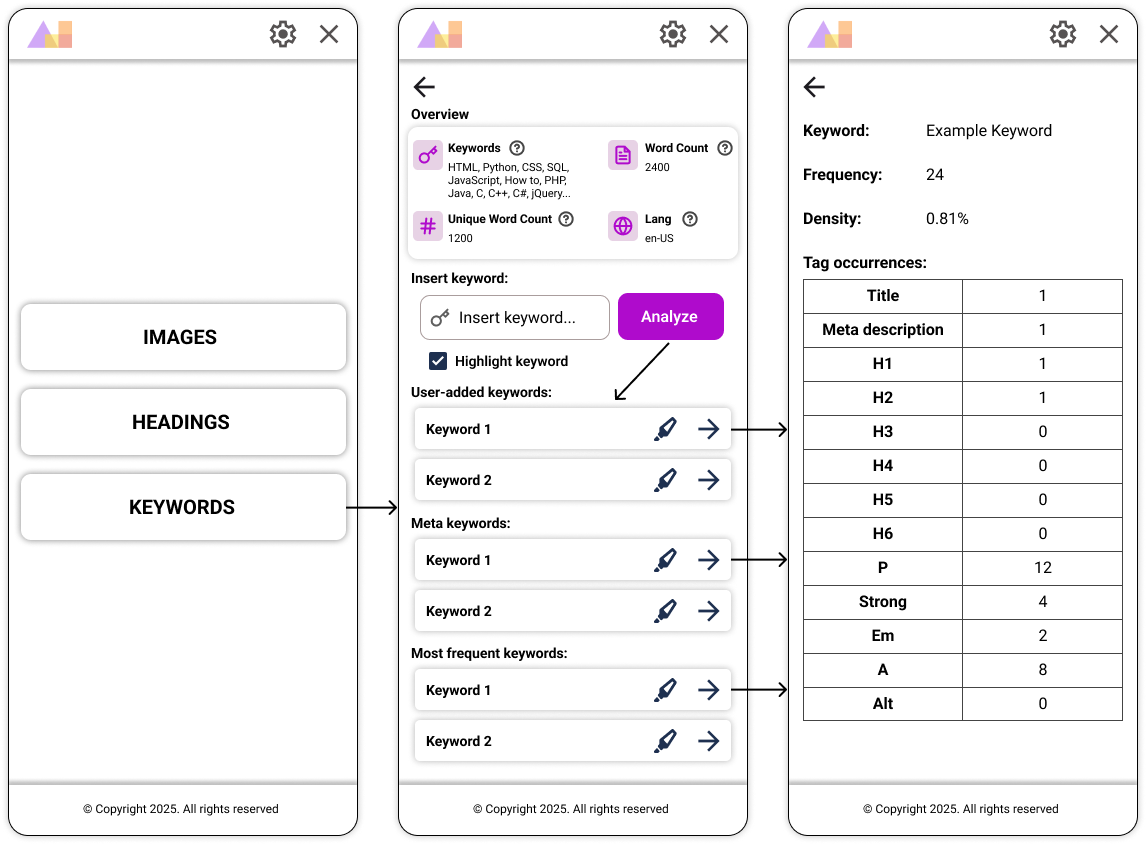
\includegraphics[width=\columnwidth]{progettazione/mockup.png} 
  \caption{Mockup dell'interfaccia grafica}
  \label{fig:mockup}
\end{figure}

\section{PoC}
\label{sec:poc}

Lo scopo principale del \gls{poc} è stato quello di tradurre in codice il \textit{mockup} dell’interfaccia grafica, al fine di verificare la correttezza e la coerenza delle scelte progettuali. Per raggiungere questo obiettivo, ho simulato il funzionamento dell’estensione in ambiente \gls{localhost}, sostituendo una pagina reale con una versione statica. Questa soluzione ha reso possibile lavorare in un ambiente di test controllato, all’interno del quale è stato possibile condurre uno studio di fattibilità e sperimentare le funzionalità di analisi e di evidenziazione visiva delle parole chiave. Al termine di questa fase, è stato organizzato un incontro con la Proponente per discutere i risultati ottenuti e le problematiche riscontrate, e identificare gli elementi da mantenere, modificare o integrare, in vista della successiva progettazione architetturale e dello sviluppo definitivo.

\section{Progettazione architetturale}
\label{sec:progettazione}

Il progetto adotta il \textit{pattern} architetturale MVC (Model-View-Controller) al fine di garantire una chiara separazione delle responsabilità tra i diversi componenti. Come illustrato in figura \ref{fig:pattern_mvc}, questo \gls{design-pattern} si articola in tre elementi principali, ciascuno con un ruolo preciso e ben definito:
\begin{itemize}
  \item \textbf{Model}: rappresenta il cuore dell’architettura. È responsabile della rappresentazione e della gestione interna dei dati, isolando le operazioni di manipolazione, archiviazione e accesso. Ha il compito di mantenere i dati organizzati, accurati e coerenti con le regole e la logica dell’applicazione;
  \item \textbf{View}: è il componente con cui l’utente interagisce direttamente. Visualizza i dati in un formato comprensibile e gestisce l’interazione tra l’utente e il sistema. Trattandosi di un componente “passivo”, la View non comunica direttamente con il Model, ma si affida al Controller per elaborare le richieste;
  \item \textbf{Controller}: funge da intermediario tra il Model e la View. Contiene la logica applicativa, elabora le richieste dell’utente e aggiorna il Model e la View di conseguenza. È responsabile della gestione del flusso dell’applicazione.
\end{itemize}

\vspace{5pt}
\noindent Il \textit{pattern} MVC promuove principi fondamentali dell'ingegneria del software, quali modularità, manutenibilità, scalabilità, robustezza e riusabilità. La chiara separazione delle responsabilità tra i componenti consente di limitare l’impatto delle modifiche, che possono essere applicate a un singolo modulo senza influire sugli altri. Inoltre, l’architettura MVC facilita l’esecuzione di test di unità e di integrazione, migliorando l’affidabilità del sistema.

\begin{figure}[H] 
  \centering 
  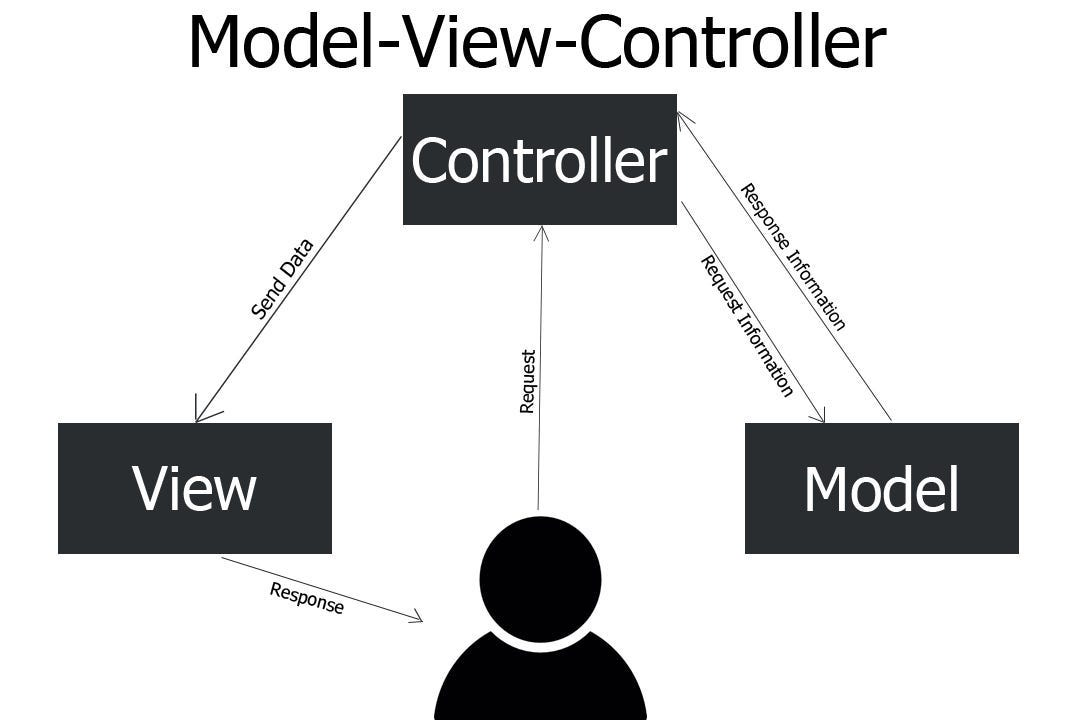
\includegraphics[width=0.6\textwidth]{progettazione/mvc.jpg} 
  \caption{Pattern MVC (Model-View-Controller)}
  \label{fig:pattern_mvc}
\end{figure}

\noindent 
\begin{minipage}{\textwidth}
  Di seguito è riportata la struttura dello strumento di analisi delle parole chiave:
  \vspace{10pt}
  \dirtree{%
    .1 .github.
    .2 workflows.
    .1 keyword.
    .2 controller.
    .2 model.
    .2 services.
    .3 strategy.
    .2 tests.
    .2 utils.
    .2 view.
    .1 static.
    .2 fonts.
    .2 img.
    .2 libs.
  }
\end{minipage}

\section{Design Pattern}
\label{sec:design-pattern}

Oltre al \textit{pattern} architetturale MVC (Model-View-Controller), ho adottato anche i \textit{pattern} Strategy e Dependency Injection.

\subsection{Strategy}

Strategy è un \gls{design-pattern} comportamentale che permette di incapsulare una famiglia di algoritmi e di selezionare dinamicamente quello più adatto. Poiché in \gls{javascript}, a differenza di linguaggi come \gls{java} o \gls{c-sharp}, non esistono interfacce in senso stretto, ho definito una classe che ne simula il comportamento all’interno del \textit{pattern} Strategy. Questa classe agisce come una struttura astratta: impedisce l'istanziazione diretta e impone l’implementazione dei metodi. Nell’ambito del progetto di stage, il \textit{pattern} Strategy è stato utilizzato per delegare una fase dell’analisi a due classi distinte, ognuna delle quali fornisce una diversa implementazione dello stesso processo. In questo modo è possibile selezionare dinamicamente l’algoritmo desiderato senza modificare il codice del modulo di analisi principale.

\vspace{10pt}
\noindent Entrambe le classi calcolano la frequenza complessiva di una parola chiave tramite la navigazione del \gls{dom} con \textit{TreeWalker}. Le differenze risiedono nel metodo utilizzato per determinare il numero di occorrenze all’interno di un insieme predefinito di tag \gls{html} ritenuti rilevanti per l’analisi. La classe \textit{StagedAnalysisStrategy} esegue un’analisi “per fasi” (staged), contando le occorrenze nei singoli tag solo dopo aver completato il calcolo della frequenza complessiva. L’algoritmo accede direttamente ai tag e ne estrae il contenuto tramite la proprietà \textit{textContent}. Al contrario, la classe \textit{AllInOneAnalysisStrategy} effettua un’analisi compatta e unificata (all in one), registrando le occorrenze nei tag contestualmente al calcolo della frequenza. In questo caso, l’accesso ai tag avviene durante la navigazione del \gls{dom}, risalendo la gerarchia (con un approccio \textit{bottom-up}) ogni volta che vengono trovati \textit{match} all’interno di un nodo.

\subsection{Dependency Injection}

Dependency Injection è un \gls{design-pattern} che consente di fornire dall’esterno le dipendenze necessarie a un oggetto, invece di istanziarle al suo interno. Le due forme di injection più comuni sono:
\begin{itemize}
  \item \textbf{Constructor Injection}: la dipendenza viene iniettata mediante il costruttore della classe;
  \item \textbf{Setter Injection}: la dipendenza viene iniettata tramite un metodo setter.
\end{itemize}

\vspace{5pt}
\noindent Il \textit{pattern} Dependency Injection favorisce un basso accoppiamento tra i componenti, promuovendo principi fondamentali dell’ingegneria del software come la flessibilità, la manutenibilità, l’estensibilità, la modularità, la riusabilità e il testing. Nell’ambito del progetto di stage, l’adozione di questo \textit{pattern} si è rivelata particolarmente utile durante la scrittura dei test di unità e di integrazione, in quanto ha permesso di sostituire le dipendenze reali con oggetti fittizi (mock).

\section{Elenco delle classi}
\label{sec:elenco-classi}

\subsection{Model}

Di seguito sono elencate le classi presenti nella cartella \textit{Model}:

\begin{itemize}
  \item \textbf{Keyword}: rappresenta il modello relativo alle parole chiave. Memorizza il nome (cioè la keyword vera e propria), la frequenza, la densità, lo stato dell’analisi e il numero di occorrenze all’interno di un insieme predefinito di tag \gls{html} considerati rilevanti per l’analisi. Espone metodi \textit{getter} e \textit{setter} per l’interazione esterna, oltre a un metodo per ripristinare lo stato del modello e uno per calcolare la densità;
  \item \textbf{KeywordListInfo}: funge da DTO (Data Transfer Object) per la View, trasportando le informazioni associate a una lista di keyword, come la categoria (es. meta keywords e user-added keywords), il titolo, le parole chiave da visualizzare, il numero totale di pagine e la modalità di ordinamento;
  \item \textbf{OverviewInfo}: memorizza le informazioni relative all’anteprima dell’analisi \gls{seo}, come il contenuto del meta tag keywords, la lingua dichiarata nella pagina, il numero totale di parole e il conteggio delle parole uniche.
\end{itemize}

\subsection{View}

Di seguito sono elencate le classi presenti nella cartella \textit{View}:

\begin{itemize}
  \item \textbf{KeywordView}: visualizza la \textit{dashboard}, ovvero il pannello di controllo principale da cui è possibile anche aggiornare l’analisi a livello globale, e gestisce le operazioni di creazione, accesso e rimozione delle sottoview. La \textit{dashboard} è suddivisa nelle seguenti sezioni:
  \begin{itemize}
    \item \textbf{Overview}: mostra un’anteprima dell’analisi \gls{seo};
    \item \textbf{Settings}: visualizza le impostazioni dell’analisi \gls{seo}, che consentono di personalizzare i colori utilizzati per evidenziare le parole chiave;
    \item \textbf{Insert Keyword}: mostra un campo di \textit{input} affiancato da un pulsante per avviare l’analisi. Include anche una \textit{checkbox}, posizionata sotto il campo di \textit{input}, che permette di attivare l’evidenziazione della parola chiave digitata;
    \item \textbf{Keyword List}: visualizza un elenco di parole chiave organizzate per categoria (es. meta keywords e user-added keywords).
  \end{itemize}
  \item \textbf{KeywordListView}: visualizza una lista di keyword suddivisa in tre sezioni virtuali:
  \begin{itemize}
    \item \textbf{Header}: mostra il titolo della lista, un campo di \textit{input} per il filtraggio delle parole chiave, due pulsanti per l’ordinamento e un pulsante per la rimozione dei filtri;
    \item \textbf{Body}: visualizza l’elenco delle parole chiave, ciascuna accompagnata da un’indicazione della frequenza e un gruppo di pulsanti per l’eliminazione, l’evidenziazione e l’accesso ai risultati dell’analisi;
    \item \textbf{Footer}: mostra l’elenco delle pagine per navigare all’interno della lista.
  \end{itemize}
  \item \textbf{AnalysisResultView}: visualizza i risultati dell’analisi di una singola parola chiave, utilizzando un formato tabellare per riportare il numero di occorrenze nei singoli tag \gls{html}. Include anche un pulsante (highlighter) che consente di evidenziare direttamente una parola chiave e che rimane sincronizzato tra tutte le View.
\end{itemize}

\subsection{Controller}

Di seguito sono elencate le classi presenti nella cartella \textit{Controller}:

\begin{itemize}
  \item \textbf{KeywordController}: si occupa dell’inizializzazione e dell’aggiornamento dell’interfaccia, dell’associazione (binding) degli eventi e della gestione delle parole chiave, includendo funzionalità come inserimento, analisi, evidenziazione, eliminazione, navigazione, ordinamento e filtraggio.
\end{itemize}

\subsection{Services}

Di seguito sono elencate le classi presenti nella cartella \textit{Services}:

\begin{itemize}
  \item \textbf{TreeWalkerManager}: gestisce la creazione dell’oggetto \textit{TreeWalker}, definendo quali nodi includere o escludere nella navigazione del \gls{dom}. Fornisce inoltre un metodo per tornare alla radice e uno per accedere al nodo successivo;
  \item \textbf{TextProcessor}: fornisce funzioni di utilità condivise dai moduli di analisi ed evidenziazione. In particolare, espone i seguenti metodi:
  \begin{itemize}
    \item \textbf{getWordsPattern}: restituisce un'espressione regolare per estrarre le parole dal testo;
    \item \textbf{getCompoundSplitPattern}: restituisce un’espressione regolare per suddividere il testo in blocchi (proposizioni);
    \item \textbf{getKeywordPattern}: restituisce un’espressione regolare per identificare una parola chiave nel testo;
    \item \textbf{getParentName}: restituisce il nome dell’elemento genitore più vicino (risalendo la gerarchia del \gls{dom} con un approccio \textit{bottom-up}), tra quelli considerati rilevanti per l’analisi;
    \item \textbf{getTextNodes}: restituisce i nodi di testo;
    \item \textbf{getTextNodeGroups}: restituisce i nodi di testo suddivisi in gruppi. Ciascun gruppo contiene nodi \textit{inline} validi (come strong ed em) che condividono lo stesso elemento genitore.
  \end{itemize}
  \item \textbf{TagAccessor}: centralizza l’accesso ai tag \gls{html} e fornisce un metodo per estrarne il contenuto testuale;
  \item \textbf{WordCounter}: si occupa di calcolare il numero di parole presenti nella pagina e di identificare quelle più frequenti. Quest’ultima operazione è gestita da due metodi distinti, \textit{findOneWordKeywords} e \textit{findCompoundKeywords}, che estraggono rispettivamente le espressioni più ricorrenti composte da una sola parola e da due o più termini (n-grammi), escludendo le \gls{stopword} in base alla lingua dichiarata nella pagina;
  \item \textbf{KeywordHighlighter}: implementa la funzionalità di evidenziazione delle parole chiave, esponendo tre metodi principali:
  \begin{itemize}
    \item \textbf{highlightKeyword}: evidenzia tutte le occorrenze di una parola chiave adottando due approcci differenti, a seconda che si tratti di una keyword semplice o di una keyphrase. Entrambi gli approcci si basano sulla stessa funzione per applicare l’evidenziazione, ma differiscono nella modalità di ricerca. Per le keyword semplici la ricerca avviene nei singoli nodi di testo, mentre per le keyphrase viene eseguita su un testo virtuale che include uno o più nodi mappati correttamente;
    \item \textbf{removeHighlight}: rimuove l’evidenziazione eseguendo una normalizzazione del \gls{dom}, al fine di ripristinare il contenuto originale;
    \item \textbf{updateTagColors}: aggiorna i colori utilizzati per l’evidenziazione delle parole chiave e inietta nuovamente lo stile nella pagina.
  \end{itemize}
  \item \textbf{KeywordAnalyzer}: implementa la funzionalità di analisi delle parole chiave, delegando al \textit{pattern} Strategy una fase del processo, che riguarda il calcolo della frequenza tramite la navigazione del \gls{dom} con \textit{TreeWalker} e la registrazione del numero di occorrenze in specifici tag \gls{html}. Questa classe espone quattro metodi principali:
  \begin{itemize}
    \item \textbf{analyzeKeyword}: esegue l’analisi di una singola parola chiave;
    \item \textbf{analyzeKeywords}: esegue l’analisi di un gruppo (batch) di parole chiave, gestendo opportunamente la \textit{cache} per ottimizzare l’esecuzione;
    \item \textbf{countOccurrencesInTag}: conta il numero di occorrenze di una parola chiave in un determinato tag;
    \item \textbf{fullRefresh}: ripristina la \textit{cache} di tutti i moduli utilizzati per l’analisi.
  \end{itemize}
\end{itemize}

\subsubsection{Strategy}

Di seguito sono elencate le classi presenti nella cartella \textit{Strategy}:

\begin{itemize}
  \item \textbf{KeywordAnalysisStrategy}: simula un’interfaccia all’interno del \textit{pattern} Strategy, definendo il contratto che le classi concrete devono implementare;
  \item \textbf{StagedAnalysisStrategy}: calcola la frequenza di una parola chiave tramite la navigazione del \gls{dom}, analizzando singoli nodi di testo o gruppi di nodi a seconda della tipologia di keyword (keyword semplice o keyphrase). I due metodi, \textit{analyzeSimpleKeyword} e \textit{analyzeCompoundKeyword}, sono richiamati dal modulo di analisi principale. Per contare il numero di occorrenze all’interno di un insieme predefinito di tag \gls{html}, entrambi i metodi analizzano direttamente i tag interessati, separatamente rispetto al calcolo della frequenza;
  \item \textbf{AllInOneAnalysisStrategy}: calcola la frequenza in modo analogo alla classe precedente. La differenza principale riguarda la modalità con cui vengono contate le occorrenze all’interno di specifici tag \gls{html}. Rispetto alla classe precedente, il conteggio avviene contestualmente al calcolo della frequenza, risalendo la gerarchia del \gls{dom} con un approccio \textit{bottom-up}. Per le keyword semplici, l’analisi viene eseguita su singoli nodi di testo; in caso di \textit{match}, è sufficiente risalire la gerarchia alla ricerca dei tag interessati e registrare le occorrenze. Per le keyphrase, invece, l’analisi si svolge su un gruppo di nodi; la registrazione delle occorrenze richiede non solo di risalire la gerarchia per individuare i tag interessati, ma anche di filtrarli per mantenere quelli comuni a tutti i nodi \textit{matchati}.
\end{itemize}

\subsection{Utils}

Di seguito sono elencate le classi presenti nella cartella \textit{Utils}:

\begin{itemize}
  \item \textbf{Utils}: fornisce due funzioni di utilità, \textit{escapeRegExp} ed \textit{escapeHTML}, che consentono rispettivamente di eseguire l’escape di un’espressione regolare e di convertire alcuni caratteri predefiniti in entità \gls{html}. 
\end{itemize}

\subsection{Tracciamento dei requisiti - Implementazione}

La tabella \ref{tab:requisiti-implementazione} riporta l’associazione tra i requisiti funzionali e le classi che ne realizzano l’implementazione.

\renewcommand{\arraystretch}{1.5}
\begin{tabularx}{\textwidth}{l >{\raggedright\arraybackslash}X l}
  \caption{Tabella dei requisiti - Implementazione}
  \label{tab:requisiti-implementazione} \\
  \hline\hline
  \textbf{Requisito} & \textbf{Classi} & \textbf{\% di copertura}\\
  \endfirsthead

  \caption[]{Tabella dei requisiti - Implementazione (continua)} \\
  \hline\hline
  \textbf{Requisito} & \textbf{Classi} & \textbf{\% di copertura} \\
  \endhead

  \multicolumn{3}{r}{{Continua nella prossima pagina}} \\
  \endfoot

  \hline
  \endlastfoot

  \hline
  RF.O.1 & \texttt{Interface} & 100\% \\
  \hline 
  RF.O.2 & \texttt{KeywordController}, \texttt{WordCounter}, \texttt{OverviewInfo}, \texttt{KeywordView} & 100\% \\
  \hline 
  RF.O.3 & \texttt{KeywordController}, \texttt{OverviewInfo}, \texttt{KeywordView} & 100\% \\
  \hline 
  RF.O.4 & \texttt{KeywordController}, \texttt{WordCounter}, \texttt{OverviewInfo}, \texttt{KeywordView} & 100\% \\
  \hline 
  RF.D.5 & \texttt{KeywordController}, \texttt{WordCounter}, \texttt{OverviewInfo}, \texttt{KeywordView} & 100\% \\
  \hline 
  RF.O.6 & \texttt{KeywordController}, \texttt{OverviewInfo}, \texttt{KeywordView} & 100\% \\
  \hline 
  RF.O.7 & \texttt{KeywordController}, \texttt{KeywordView}, \texttt{KeywordListView} & 100\% \\
  \hline 
  RF.O.8 & \texttt{KeywordController}, \texttt{KeywordAnalyzer}, \texttt{StagedAnalysisStrategy}, \texttt{AllInOneAnalysisStrategy}, \texttt{Keyword}, \texttt{KeywordView}, \texttt{KeywordListView} & 100\% \\
  \hline 
  RF.O.9 & \texttt{KeywordController}, \texttt{Keyword}, \texttt{KeywordListInfo}, \texttt{KeywordView}, \texttt{KeywordListView} & 100\% \\
  \hline 
  RF.O.10 & \texttt{KeywordController}, \texttt{Keyword}, \texttt{KeywordListInfo}, \texttt{KeywordView}, \texttt{KeywordListView} & 100\% \\
  \hline 
  RF.O.11 & \texttt{KeywordController}, \texttt{Keyword}, \texttt{KeywordListInfo}, \texttt{KeywordView}, \texttt{KeywordListView} & 100\% \\
  \hline 
  RF.OP.12 & \texttt{KeywordController}, \texttt{WordCounter}, \texttt{Keyword}, \texttt{KeywordListInfo}, \texttt{KeywordView}, \texttt{KeywordListView} & 100\% \\
  \hline 
  RF.OP.13 & \texttt{KeywordController}, \texttt{WordCounter}, \texttt{Keyword}, \texttt{KeywordListInfo}, \texttt{KeywordView}, \texttt{KeywordListView} & 100\% \\
  \hline 
  RF.OP.14 & \texttt{KeywordController}, \texttt{WordCounter}, \texttt{Keyword}, \texttt{KeywordListInfo}, \texttt{KeywordView}, \texttt{KeywordListView} & 100\% \\
  \hline 
  RF.O.15 & \texttt{KeywordController}, \texttt{Keyword}, \texttt{KeywordListInfo}, \texttt{KeywordView}, \texttt{KeywordListView} & 100\% \\
  \hline 
  RF.O.16 & \texttt{KeywordController}, \texttt{KeywordHighlighter}, \texttt{Keyword}, \texttt{KeywordView} & 100\% \\
  \hline 
  RF.O.17 & \texttt{KeywordController}, \texttt{Keyword}, \texttt{AnalysisResultView} & 100\% \\
  \hline 
  RF.D.18 & \texttt{KeywordController}, \texttt{Keyword}, \texttt{KeywordView}, \texttt{KeywordListView} & 100\% \\
  \hline 
  RF.O.19 & \texttt{KeywordController}, \texttt{Keyword}, \texttt{KeywordListInfo}, \texttt{KeywordView}, \texttt{KeywordListView}, \texttt{AnalysisResultView} & 100\% \\
  \hline 
  RF.O.20 & \texttt{KeywordController}, \texttt{Keyword}, \texttt{KeywordListInfo}, \texttt{KeywordView}, \texttt{KeywordListView}, \texttt{AnalysisResultView} & 100\% \\
  \hline 
  RF.O.21 & \texttt{KeywordController}, \texttt{Keyword}, \texttt{KeywordView}, \texttt{AnalysisResultView} & 100\% \\
  \hline 
  RF.O.22 & \texttt{KeywordController}, \texttt{Keyword}, \texttt{KeywordView}, \texttt{AnalysisResultView} & 100\% \\
  \hline 
  RF.O.23 & \texttt{KeywordController}, \texttt{Keyword}, \texttt{KeywordView}, \texttt{AnalysisResultView} & 100\% \\
  \hline 
  RF.O.24 & \texttt{KeywordController}, \texttt{Keyword}, \texttt{KeywordView}, \texttt{AnalysisResultView} & 100\% \\
  \hline 
  RF.O.25 & \texttt{KeywordController}, \texttt{Keyword}, \texttt{KeywordView}, \texttt{AnalysisResultView} & 100\% \\
  \hline 
  RF.D.26 & \texttt{KeywordController}, \texttt{Keyword}, \texttt{KeywordView}, \texttt{KeywordListView} & 100\% \\
  \hline 
  RF.D.27 & \texttt{KeywordController}, \texttt{Keyword}, \texttt{KeywordView}, \texttt{KeywordListView} & 100\% \\
  \hline 
  RF.D.28 & \texttt{KeywordController}, \texttt{Keyword}, \texttt{KeywordView}, \texttt{KeywordListView} & 100\% \\
  \hline 
  RF.O.29 & \texttt{KeywordController}, \texttt{Keyword}, \texttt{KeywordView}, \texttt{KeywordListView} & 100\% \\
  \hline 
  RF.OP.30 & \texttt{KeywordController}, \texttt{WordCounter}, \texttt{KeywordAnalyzer}, \texttt{StagedAnalysisStrategy}, \texttt{AllInOneAnalysisStrategy}, \texttt{Keyword}, \texttt{OverviewInfo}, \texttt{KeywordView}, \texttt{KeywordListView} & 100\% \\
  \hline 
  RF.O.31 & \texttt{KeywordController}, \texttt{OverviewInfo}, \texttt{KeywordView} & 100\% \\
  \hline 
  RF.O.32 & \texttt{KeywordController}, \texttt{OverviewInfo}, \texttt{KeywordView} & 100\% \\
  \hline 
  RF.O.33 & \texttt{KeywordController}, \texttt{Keyword}, \texttt{KeywordListInfo}, \texttt{KeywordView}, \texttt{KeywordListView}, \texttt{AnalysisResultView} & 100\% \\
  \hline 
  RF.O.34 & \texttt{KeywordController}, \texttt{Keyword}, \texttt{KeywordView}, \texttt{AnalysisResultView} & 100\% \\
  \hline 
  RF.OP.35 & \texttt{KeywordController}, \texttt{KeywordHighlighter}, \texttt{KeywordView} & 100\% \\
  \hline 
  RF.OP.36 & \texttt{KeywordController}, \texttt{KeywordHighlighter}, \texttt{KeywordView} & 100\% \\
  \hline 
  RF.OP.37 & \texttt{KeywordController}, \texttt{KeywordHighlighter}, \texttt{KeywordView} & 100\% \\
  \hline 
  RF.OP.38 & \texttt{KeywordController}, \texttt{KeywordHighlighter}, \texttt{KeywordView} & 100\% \\
  \hline 
  RF.O.39 & \texttt{KeywordController}, \texttt{KeywordAnalyzer}, \texttt{StagedAnalysisStrategy}, \texttt{AllInOneAnalysisStrategy}, \texttt{Keyword} & 100\% \\
  \hline 
  RF.OP.40 & \texttt{KeywordController}, \texttt{KeywordAnalyzer}, \texttt{StagedAnalysisStrategy}, \texttt{AllInOneAnalysisStrategy}, \texttt{Keyword} & 100\% \\
  \hline 
  RF.O.41 & \texttt{KeywordHighlighter} & 100\% \\
  \hline 
  RF.OP.42 & \texttt{WordCounter} & 100\% \\
  \hline 
  RF.D.43 & \texttt{WordCounter}, \texttt{KeywordAnalyzer}, \texttt{StagedAnalysisStrategy}, \texttt{AllInOneAnalysisStrategy}, \texttt{KeywordHighlighter} & 100\% \\
\end{tabularx}